
\subsection{State Function}
A function that describes the \emph{equilibrium} state of a system, irrespective of how the system
arrived in the state. e.g, $f(p,V,T)=0$. Whereas, mechnical work and heat depends on the \emph{path}
between two equilibrium states. \\

\subsection{Ideal gas}
For $n$ moles of any gas
\begin{equation}
    pV = nR^*T,
\end{equation}
with the universal constant $R^*$ [$J K^{-1}$ mol$^{-1}$]. We know that $n=1$ mole of dry air equals
$M_d$ (molecular weight for dry air) grams of dry air, $1[\text{mol}] = M_d [0.001\text{kg}]$,
\begin{equation}
        p_d V_d  = M_d \Big(\frac{1000 R^*}{M_d} [ J K^{-1} \text{kg}^{-1}]\Big) T \\
\end{equation}
which becomes
\begin{equation} \label{eq:idealgas2}
    p_d \alpha_d = R_d T.
\end{equation}
This is the general relationship of any gas, hence the water vapor pressure 
\begin{equation} \label{eq:idealgas3}
   e \alpha_v = R_v T.
\end{equation}

\subsection{Thermodynamic equation}
\begin{equation}
    \frac{DI}{Dt} + p \frac{D\alpha}{Dt} = \dot{Q}
\end{equation}
Q. How to relate the pressure (state) in the momentum equation by the thermodynamic equation? \\
A. $dI = c_v dT \Rightarrow I = c_v T$, and assuming ideal gas $p = \rho R T \Rightarrow p = \rho R
I / c_v$,
hence,
\begin{equation}
    \frac{DI}{Dt} - \frac{p}{\rho^2} \frac{D\rho}{Dt} = \dot{Q},
\end{equation}
with the continuity equation it becomes
\begin{equation}
    \frac{DI}{Dt} + \frac{p}{\rho} \nabla \cdot v = \dot{Q}.
\end{equation}
Q. Assuming large scale in \emph{hydrostatic balance}? \\
A. $\alpha d p = -gdz$, hence $dQ = c_v dT - \alpha dp = c_v dT + gdz = d(c_v T + gz) = ds$ (dry
static energy)
\begin{equation}
    \frac{Ds}{Dt} = \dot{Q}.
\end{equation}
Q. What about general gas (non-ideal)? \\
A. Diagnostic equation for pressure is $p = -\frac{\partial I}{\partial \alpha}$. \\

\subsection{Entropy}
A measure of ``difference'' between adiabats (no heat exchange processes), and a measure of ``work
loss'' in transferring heat (irreversible process). \\

In a closed system, when heat is added at a constant temperature (volume expands and pressure
decreases), the amount of disorder increases which increases the potential temperature (the actual
temperature is higher when forced back to original pressure). For a irreversible process, suppose a
heat reservoir at $T_2$ transfers heat $Q$ to a cooler reservoir at $T_0$. By Carnot's engine, we
know that the maximum available energy the heat tranferred into work is
\begin{equation}
    W_2 = (1-\frac{T_0}{T_2})Q.
\end{equation}

For a irreversible process (state variables (e.g., p, V, T) cannot go back to original values
without additional work), where heat is first transferred to a middle reservoir at the state $T_1 <
T_2$, and then transfers the same amount of heat $Q$ to the cold reservoir at $T_0$.
Notice since $T_1 < T_2$, therefore the entropy is higher to transfer the same amount of $Q$.
Therefore the maximum available work from the middle reservoir is
\begin{equation}
    W_1 = (1-\frac{T_0}{T_1})Q,
\end{equation}
which is less than $W_2$. Hence, the work loss from irreversible process is 
\begin{equation}
    W_2-W_1 = Q(T_0/T_1 - T_0/T_2) = T_0(S_1 - S_2) = T_0 dS,
\end{equation} 
in a form of heat loss, where the increase in $dS$ becomes a measure of work loss. 
%A sum of entropy gain of $S_1$ from the middle reservoir and 
%entropy loss of $S_2$ from the original reservoir in the irreversible process.
There is a net gain in entropy in the irreversible process.
i.e., {\bf the more entropy gain/more disorderness contributes to more work loss, which becomes a
less efficient process.}

\subsection{specific volume}
{\bf Definition}: $v = 1/\rho$, volume occupied by 1kg of mass.

\subsection{latent heat}
{\bf Definition}: $Q_l$, energy released/absorbed by a body during a constant temperature process
(phase transition).


\subsection{Clausius-Claperon Relation}
{\bf Definition}: $\frac{\Delta P}{\Delta T} = \frac{L}{T\Delta v}$, P-T coexistence curve slope
relation. Under typical atmoshperic conditions, 
\begin{equation}
   \frac{d e_s}{dT} = \frac{L_v(T)e_s}{R_vT^2}, 
\end{equation}
where: $L_v$ is latent heat for evaporation varying with $T$, $R_v$ is the water vapor gas constant.
\\


\subsection{saturation vapor pressure}
\noindent August-Roche-Magnus formula (approximation from Clausius-Claperon Relation): \\
\begin{equation}
   e_s(T) = 6.1094 \text{exp}(\frac{17.625T}{T+243.04}).
\end{equation}
( water-holding capacity of the atmosphere increases by about $7\%$ for every $1^{\circ}$C rise in
temperature )

\subsection{unsaturated vapor pressure}
{\bf Definition}: $e = \frac{(n_{\text{air}} + n_{\text{water}})}{V}RT$, 

\subsection{relative humidity}
{\bf Definition}: $RH = \frac{e}{e_s}(T)$.

\subsection{virtual temperature}
{\bf Purpose}:
The gas constant for moist air (a mix of pure water vapor and dry air) depends strongly on the
amount of water vapor, so it is convenient to use a fictitious temperature with the dry-air equation
of state to represent how "heavy" a moist parcel is (i.e., the more water vapor means a dry air
needs to rise more to reach same pressure and density to become "light"). \\

{\bf Definition}: $T_v = T_\text{dry}(P,\rho)$, temperature at which a dry parcel would have a
pressure and density equal to the moist parcel. \\

{\bf Derivation}: Suppose a moist parcel has density $\rho$ and pressure $p$.
Dalton's law of partial pressure gives $p = e + p_d$, combined with \eqref{eq:idealgas2} and
\eqref{eq:idealgas3} give
\begin{equation}
   \rho = \frac{m_d + m_v}{V} = \rho_d + \rho_v = \frac{p-e}{R_dT} + \frac{e}{R_vT}, 
\end{equation}
where $\rho_d$ and $\rho_v$ are the partial densities.
Solving this gives
\begin{equation}
   p = \rho R_d \frac{T}{1-\frac{e}{p}(1-\frac{R_d}{R_v})} = \rho R_d T_v,
\end{equation}
where, $\frac{R_d}{R_v} \approx 0.622$ in the atmosphere. \\

\subsection{lifting condensation level (LCL)}
{\bf Definition}: $h_{LC}$, height at which an unsaturated parcel reaches saturation, $RH=100\%$, dry
adiabatically, then starts following moist adiabatic lapse rate upward. 
\begin{figure} [H] 
   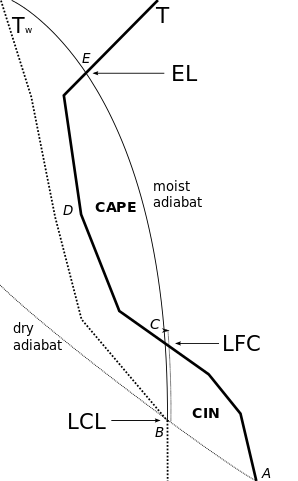
\includegraphics[width=0.2\textwidth, height=0.3\textwidth]{sounding.png}
   \caption{\label{sounding}}
\end{figure}

\subsection{level of free convection (LFC)}
{\bf Definition}: $h_{FC}$, height at which a moist parcel temperature is equal to the environment,
and temperature increases faster than the environment. \\

{\bf Example}: The unsaturated parcel in Figure {\ref{sounding}} is lifted dry adiabatically from A
to B to saturation, and further lifted moist adiabatically to C until surpassing the environmental
temperature.

\subsection{dew point temperature}
{\bf Definition}: $T_d$, temperature at LCL when a parcel reaches $RH=100\%$.

\subsection{convective inhibition (CIN)}
{\bf Definition}: CIN $=\int_{h_0}^{h_{FC}} g \frac{T_{v,\text{parcel}}-T_{v,\text{env}}}{T_{v,\text{env}}} dz$, 
a negative energy value measuring how much a parcel is prevented to rise to LFC from the surface. \\
{\bf Interpretation}: The term $\frac{T_{v,\text{parcel}}}{T_{v,\text{env}}} -
1$ shows when the parcel is moister (larger $T_{v,\text{parcel}}$, more buoyant), CIN is less negative.


\subsection{
